\section{Introduction}

In this chapter I apply the OmniTune framework to SkelCL. The publicly
available implementation
\footnote{\url{https://github.com/ChrisCummins/omnitune}} predicts
workgroup sizes for OpenCL stencil skeleton kernels in order to
minimise their runtime on CPUs and multi-GPU systems. The optimisation
space presented by the workgroup size of OpenCL kernels is large,
complex, and non-linear. Successfully applying machine learning to
such a space requires plentiful training data, the careful selection
of features, and classification approach. The following sections
address these challenges.


% Anyone downloading a copy of OmniTune will instantly have access to
% the global database of training data, including the
% \input{gen/num_samples} runtimes which were collected to write this
% thesis.

% \texttt{cec.chlox1mra3iz.us-west-2.rds.amazonaws.com:3306}

\section{Training}\label{sec:training}

One challenge of performing empirical performance evaluations is
gathering enough applications to ensure meaningful
comparisons. Synthetic benchmarks are a popular method for
circumventing this problem. The automatic generation of such
benchmarks has clear benefits for reducing evaluation costs; however,
creating meaningful benchmark programs is a difficult problem if we
are to avoid the problems of redundant computation and produce
provable halting benchmarks.

In practise, stencil codes exhibit many common traits: they have a
tightly constrained interface, predictable memory access patterns, and
well defined numerical input and output data types. This can be used
to create a confined space of possible stencil codes by enforcing
upper and lower bounds on properties of the codes which can not
normally be guaranteed for general-purpose programs, e.g.\ the number
of floating point operations. In doing so, it is possible to
programatically generate stencil workloads which share similar
properties to those which we intend to target.

Based on observations of real world stencil codes from the fields of
cellular automata, image processing, and PDE solvers, I implemented a
stencil generator which uses parameterised kernel templates to produce
source codes for collecting training data. The stencil codes are
parameterised by stencil shape (one parameter for each of the four
directions), input and output data types (either integers, or single
or double precision floating points), and \emph{complexity} --- a
simple boolean metric for indicating the desired number of memory
accesses and instructions per iteration, reflecting the relatively
bi-modal nature of the reference stencil codes, either compute
intensive (e.g. FDTD simulation), or lightweight (e.g. Game of Life).

Using a large number of synthetic benchmarks helps adress the ``small
$n$, large $P$'' problem, which describes the difficulty of
statistical inference in spaces for which the set of possible
hypotheses $P$ is significantly larger than the number of observations
$n$\CitationNeeded{}. By creating parameterised, synthetic benchmarks,
it is possible to explore a much larger set of the space of possible
stencil codes than if relying solely on reference applications,
reducing the risk of overfitting to particular program features.


\section{Stencil Features}


\begin{table}
\begin{multicols}{2}
\scriptsize
\centering
\rowcolors{2}{white}{gray!25}
\begin{multicols}{2}
\scriptsize
\centering
\rowcolors{2}{white}{gray!25}
\begin{multicols}{2}
\scriptsize
\centering
\rowcolors{2}{white}{gray!25}
\input{gen/tab/features.1}
\vfill
\columnbreak
\rowcolors{2}{white}{gray!25}
\input{gen/tab/features.2}
\end{multicols}

\vfill
\columnbreak
\rowcolors{2}{white}{gray!25}
\begin{multicols}{2}
\scriptsize
\centering
\rowcolors{2}{white}{gray!25}
\input{gen/tab/features.1}
\vfill
\columnbreak
\rowcolors{2}{white}{gray!25}
\input{gen/tab/features.2}
\end{multicols}

\end{multicols}

\vfill
\columnbreak
\rowcolors{2}{white}{gray!25}
\begin{multicols}{2}
\scriptsize
\centering
\rowcolors{2}{white}{gray!25}
\begin{multicols}{2}
\scriptsize
\centering
\rowcolors{2}{white}{gray!25}
\input{gen/tab/features.1}
\vfill
\columnbreak
\rowcolors{2}{white}{gray!25}
\input{gen/tab/features.2}
\end{multicols}

\vfill
\columnbreak
\rowcolors{2}{white}{gray!25}
\begin{multicols}{2}
\scriptsize
\centering
\rowcolors{2}{white}{gray!25}
\input{gen/tab/features.1}
\vfill
\columnbreak
\rowcolors{2}{white}{gray!25}
\input{gen/tab/features.2}
\end{multicols}

\end{multicols}

\end{multicols}

\caption{Stencil features and their types, describing the dataset, kernel,
  and device.}
\label{tab:features}
\end{table}


Properties of the architecture, program, and dataset all contribute to
the performance of a workgroup size. The success of a machine learning
system depends on the ability to translate these properties into
meaningful explanatory variables --- \emph{features}. To capture this
in OmniTune, requests for paramters are packed with a copy of the
OpenCL kernel and attributes of the dataset and device to extract
vectors of 102 features describing hte architecture, kernel, and
dataset. Table~\ref{tab:features} includes a full list of features and
types.


\begin{itemize}
\item \textbf{Device} --- OmniTune uses the OpenCL
  \texttt{clGetDeviceInfo()} API to query a number of properties about
  the target execution device. Examples include the size of local
  memory, maximum work group size, number of compute units, etc.
\item \textbf{Kernel} --- The user code for a stencil is passed to the
  OmniTune server, which compiles the OpenCL kernel to LLVM IR
  bitcode. The \texttt{opt} \texttt{InstCount} statistics pass is used
  to obtain static counts for each type of instruction present in the
  kernel, as well as the total number of instructions. The instruction
  counts for each type are divided by the total number of instructions
  to produce a \emph{density} of instruction for that type. Examples
  include total static instruction count, ratio of instructions per
  type, ratio of basic blocks per instruction, etc.
\item \textbf{Dataset} --- The SkelCL container type is used to
  extract the input and output data types, and the 2D grid size.
\end{itemize}


\subsection{Reducing Feature Extraction Overhead}


Feature extraction (particularlly compilation to LLVM IR) introduces a
runtime overhead to the classification process. To minimise this,
lookup tables for device and dataset features are used, and cached
locally in the OmniTune server and pushed to the remote data
store. The device ID is used to index the devices table, and the
checksum of an OpenCL source is used to index the kernel features
table. Before feature extraction for either occurs, a lookup is
performed in the relevant table, meaning that the cost of feature
extraction is amortised over time.


\section{Optimisation Parameters}\label{sec:op-params}

SkelCL stencil kernels are parameterised by a workgroup size $w$,
which consists of two integer values to denote the number of rows and
columns (where we need to distinguish the individual components, we
will use symbols $w_r$ and $w_c$ to denote rows and columns,
respectively).


\subsection{Constraints}

Unlike in many autotuning applications, the space of optimisation
parameter values is subject to hard constraints, and these constraints
cannot conviently be statically determined. Contributing factors are
architectural limitations, kernel constraints, and refused parameters.


\subsubsection{Architectural constraints}

Each OpenCL device imposes a maximum workgroup size which can be
statically checked by querying the \texttt{clGetDeviceInfo()} API for
that device. These are defined by archiectural limitations of how code
is mapped to the underlying execution hardware. Typical values are
powers of two, e.g.\ 1024, 4096, 8192.


\subsubsection{Kernel constraints}

At runtime, once an OpenCL program has been compiled to a kernel,
users can query the maximum workgroup size supported by that kernel
using the \texttt{clGetKernelInfo()} API. This value cannot easily be
obtained statically as there is no mechanism to determine the maximum
workgroup size for a given source code and device without first
compiling it, which in OpenCL does not occur until runtime. Factors
which affect a kernel's maximum workgroup size include the number
registers required for a kernel, and the available number of SIMD
execution units for each type of instructions in a kernel.


\subsubsection{Refused parameters}

\TODO{\ldots}


\subsubsection{Legality}

We define a \emph{legal} workgroup size as one which, for a given
\emph{scenario} (a combination of program, device, and dataset),
satisfies the architectural and kernel constraints, and is not
refused. The subset of all possible workgroup sizes
$W_{legal}(s) \subset W$ that are legal for a given sceanario $s$ is
then:
%
\begin{equation}
  W_{legal}(s) = \left\{w | w \in W, w < W_{\max}(s) \right\} - W_{refused}(s)
\end{equation}
%
Where $W_{\max}(s)$ can be determined at runtime prior to the kernels
execution, but the set $W_{refused}(s)$ can only be determined
experimentally. Exceeding either of these constraints will cause an
\texttt{CL\_OUT\_OF\_RESOURCES} error when the OpenCL kernel is
enqueued.


\subsection{Assessing Relative Performance}

Given a set of observations of observed runtime for $(s,w)$ pairs, and
a function $t(s,w)$ which returns the arithmetic mean of the observed
runtimes for a pair, we can calculate the speedup $r(s, w_1, w_2)$ of
competing workgroup sizes $w_1$ over $w_2$ using:
%
\begin{equation}
  r(s, w_1, w_2) = \frac{t(s,w_2)}{t(s,w_1)}\\
\end{equation}
%

\subsubsection{Oracle Workgroup Size}

The \emph{oracle} workgroup size $\Omega(s) \in W_{legal}(s)$ of a
sceanrio $s$ is the $w$ value which provides the lowest mean
runtime. This allows for comparing the performance $p(s,w)$ of a
particular workgroup against the maximum available performance for
that scenario, within the range $0 \le p(s,w) \le 1$:

\begin{align}
  \Omega(s) &= \argmin_{w \in W_{legal}(s)} t(s,w)\\
  p(s,w) &= r(s, w, \Omega(s))
\end{align}


\subsubsection{Establishing a Baseline}

The geometric mean is used to aggregate normalised relative
performances due to its multiplicative
property~\cite{Fleming1986}. For a given workgroup size, the average
performance $\bar{p}(w)$ across the set of all scenarios $S$ can be
found using the geometric mean of performance relative to the oracle:
%
\begin{equation}
\bar{p}(w) =
\left(
  \prod_{s \in S} r(s, w, \Omega(s))
\right)^{1/|S|}
\end{equation}
%
The \emph{baseline} workgroup size $\bar{w}$ is the value which
provides the best average case performance across all scenarios. Such
a baseline value represents the \emph{best} possible performance which
can be achieved using a single, statically chosen workgroup size. By
defining $W_{safe} \in W$ as the intersection of legal workgroup
sizes, the baseline can be found using:

\begin{align}
W_{safe} &= \cap \left\{ W_{legal}(s) | s \in S \right\}\\
\bar{w} &= \argmax_{w \in W_{safe}} \bar{p}(w)
\end{align}


\section{Machine Learning}

The challenge is to design a system which, given a set of prior
observations of the empirical performance of stencil codes with
different workgroup sizes, predict workgroup sizes for \emph{unseen}
stencils which will maximise the performance. The OmniTune server
supports three methods for achieving this.


\subsection{Predicting Oracle Workgroup Size}

The first approach to predicting workgroup sizes is to consider the
set of possible workgroup sizes as a hypothesis space, and to use a
classifier to predict, for a given set of features, the workgroup size
which will provide the best performance. The classifier takes a set of
training scenarios $S_{training}$, and generates labelled training
data as pairs of scenario features $f(s)$ and observed oracle
workgroup sizes:
%
\begin{equation}
  T = \left\{ \left(f(s), \Omega(s)\right) | s \in S_{training} \right\}
\end{equation}
%
During testing, the classifier predicts workgroup sizes from the set
of oracle workgroup sizes from the training set:
%
\begin{equation}
  W_{training} = \left\{ \Omega(s) | s \in S_{training} \right\}
\end{equation}
%
This approach presents the problem that after training, there is no
guarantee that the set of workgroup sizes which may be predicted is
within the set of legal workgroup sizes for future scenarios:
%
\begin{equation}
  \cup \{ W_{legal}(s) | s \in S_{testing} \} \nsubseteq W_{training}
\end{equation}
%
This may result in a classifier predicting a workgroup size which is
not legal for a scenario, $w \not\in W_{legal}(s)$, either because it
exceeds $W_{\max}(s)$, or because the parameter is refused. For these
cases, I evaluate the effective of three fallback strategies to select
a legal workgroup size:

\begin{enumerate}
\item \emph{Baseline} --- select the workgroup size which is known to
  be safe $w < W_{safe}$, and provides the highest average case
  performance on training data.
\item \emph{Random} --- select a random workgroup size which is known
  from prior observations to be legal $w \in W_{legal}(s)$.
\item \emph{Nearest Neighbour} --- select the workgroup size which
  from prior observations is known to be legal, and has the lowest
  Euclidian distance to the prediction.
\end{enumerate}

See Algorithm~\ref{alg:autotune-classification} for definitions.

\begin{algorithm}
\begin{algorithmic}[1]
\Require kernel features $k$, hardware features $h$, dataset features
$d$.
\Ensure workgroup size $w$

\Procedure{Default}{w, a, k, d}
\Comment Use the best safe param.
\State $w \leftarrow \text{classify}(a, k, d)$
\If{$w \in W_{legal}(s)$}
    \State \textbf{return} $w$
\Else
  \State \textbf{return} $\underset{w \in W_{safe}}{\argmax}
\left(
  \prod_{s \in S_{training}} p(s, w)
\right)^{1/|S_{training}|}$
\EndIf
\EndProcedure
\item[]

\Procedure{Random}{w, a, k, d}
\Comment Use a random param from $W_{legal}$.
\State $w \leftarrow \text{classify}(a, k, d)$
\If{$w \in W_{legal}(s)$}
    \State \textbf{return} $w$
\Else
  \State \textbf{return} random choice $w \in W_{legal}$
\EndIf
\EndProcedure
\item[]

\Procedure{Reshape}{w, a, k, d}
\Comment Coerce params to be legal.
\State $w \leftarrow \text{classify}(a, k, d)$
\If{$w \in W_{legal}(s)$}
    \State \textbf{return} $w$
\Else
  \State $d_{min} \leftarrow \infty$
  \State $w_{closest} \leftarrow \text{null}$
  \For{$c \in W_{legal}$}
    \State $d \leftarrow \sqrt{\left(c_r - w_r\right)^2 + \left(c_c - w_c\right)^2}$
    \If{$d < d_{min}$}
      \State $d_{min} \leftarrow d$
      \State $w_{closest} \leftarrow c$
    \EndIf
  \EndFor
  \State \textbf{return} $w_{closest}$
\EndIf
\EndProcedure
\end{algorithmic}

\caption{Select optimal workgroup size using classification}
\label{alg:autotune-classification}
\end{algorithm}

% \begin{algorithm}
% \begin{algorithmic}[1]
\Require kernel features $k$, hardware features $h$, dataset features
$d$.
\Ensure workgroup size $w$

\State $C \leftarrow \phi$
\Comment Set of classifiers.
\State $W_{training} \leftarrow \{ W_{legal}(s) | s \in S_{training}
\}$

\For{$W_c \in W_{training}$}
  \State $S_c \leftarrow \{ s | s \in S_{training}, W_{legal}(s) = W_c
  \}$
  \Comment Training data with same legal params.
  \State $c \leftarrow \text{\sc{TrainClassifier}}(S_c)$
  \Comment Build a classifier with training data.
  \State $C \leftarrow C \cup \{ c \}$
\EndFor

\State $c \leftarrow C_{W_{legal}(s)}$

\State \textbf{return} $c(a, k, d)$
\end{algorithmic}

% \caption{Select optimal workgroup size using multiple classifiers}
% \label{alg:autotune-classification2}
% \end{algorithm}


\subsection{Predicting Stencil Code Runtime}

A problem of predicting oracle workgroup sizes is that it requires
each training point to be labelled with the oracle workgroup size
which can be only be evaluated using an exhaustive search. An
alternative approach is to build a model to attempt to predict the
\emph{runtime} of a stencil given a specific workgroup size. This
allows for training on data for which the oracle workgroup size is
unknown. Given training data consisting of $(f(s),w,t)$ tuples, where
$s$ is scenario, $w$ is the workgroup size, and $t$ is the observered
mean runtime, we can train a regressor $g(f(s), w)$ which predicts the
mean runtime of an unseen scenario. The predicted oracle workgroup
size $\bar{\Omega}(s)$ is then $w$ value which minimises the output of
the regressor:
%
\begin{equation}
  \bar{\Omega}(s) = \underset{w \in W_{legal}(s)}{\argmin} g(f(s), w)
\end{equation}
%
By predicting the runtimes of only the workgroup sizes from within
$W_{legal}(s)$, we overcome the issue of predicting workgroup sizes
which exceed $W_{\max}(s)$, although note that since $W_{refused}(s)$
is immergent, it may still be possible predict invalid workgroup sizes
unseen programs.

% \begin{algorithm}
% \begin{algorithmic}[1]
\Require kernel features $k$, hardware features $h$, dataset features
$d$.
\Ensure predicted oracle workgroup size $\bar{\Omega}(s)$
\State $C \leftarrow \{c_1, c_2, \ldots, c_n \}$
\Comment Set of all workgroup sizes $\le k.\text{max\_wgsize}$
\State \textbf{return} $\underset{c \in C}{\argmin} f(k,h,d,c)$
\end{algorithmic}

% \caption{Selecting workgroup size using runtime regression}
% \label{alg:autotune-runtime-regression}
% \end{algorithm}

\subsection{Predicting Relative Performance of Workgroup Sizes}

Accurately predicting the runtime of an arbitrary program is a
difficult problem due to the impacts of flow control. In such cases,
it may be more effective to instead predict the \emph{relative}
performance of two different workgroup sizes for the same program. To
do this, we select a baseline workgroup size $w_b \in W_{safe}$, and
train a regressor $g(f(s),w,w_b)$ with training data labelled with the
relative performance over the baseline $r(w, w_b)$. Predicting the
optimal workgroup requires maximising the output of the regressor:
%
\begin{equation}
  \bar{\Omega}(s) = \underset{w \in W_{legal}(s)}{\argmax} g(f(s),w,w_b)
\end{equation}
%

% \begin{algorithm}
% \begin{algorithmic}[1]
\Require kernel features $k$, hardware features $h$, dataset features
$d$.
\Ensure workgroup size $w$
\State $C \leftarrow \{c_1, c_2, \ldots, c_n \}$
\Comment Set of all workgroup sizes $\le k.\text{max\_wgsize}$
\State \textbf{return} $\underset{c \in C}{\argmax} f(k,h,d,c)$
\end{algorithmic}

% \caption{Selecting workgroup size using speedup regression}
% \label{alg:autotune-speedup-regression}
% \end{algorithm}


\subsection{Meta-tuning: a Hybrid Approach}

\TODO{Implement and test. See Algorithm~\ref{alg:autotune-hybrid}.}

\begin{algorithm}
\begin{algorithmic}[1]
\Require kernel features $k$, hardware features $h$, dataset features $d$.
\Ensure workgroup size $w$

\State $r \leftarrow \underset{w \in W_{legal}(s)}{\min} f(k,h,d,w)$
\Comment Predict minimum runtime.
\State $w \leftarrow \underset{w \in W_{legal}(s)}{\argmin} f(k,h,d,w)$
\Comment Workgroup size for $r$.
\State $t_r \leftarrow$ measure runtime of program with $w$
\If{$t_r \approx r$}
  \State \textbf{return} $w$
\Comment Predicted runtime is accurate.
\Else
   \State $W \leftarrow W_{legal}(s)$
   \State converged $\leftarrow$ false
   \State $w_b \leftarrow$ baseline value
   \State $t_b \leftarrow$ measure runtime of runtime of program with $w_b$
   \While{not converged}
     \State $s \leftarrow \underset{w \in W}{\max} g(k,h,d,w)$
     \Comment Predict best speedup.
     \State $w \leftarrow \underset{w \in W}{\argmax} g(k,h,d,w)$
     \Comment Workgroup size for $s$.
     \State $t \leftarrow$ measure runtime of program with $s$
     \If{$t_b / t \approx s$}
       \State converged = true
       \Comment Predicted speedup is accurate.
     \Else
       \State $W = W - \{w\}$
     \EndIf
   \EndWhile
   \State \textbf{return} $w$
\EndIf
\end{algorithmic}

\caption{Selecting workgroup size using a hybrid approach}
\label{alg:autotune-hybrid}
\end{algorithm}


\section{Implementation}

By design, the client-server model minimises the impact of number of
modifications that are required to enable autotuning in client
applications. The only modification required is to replace the
hardcoded values for workgroup size with a subroutine to request a
workgroup size from the OmniTune server over a DBUS connection.

The server is implemented as a standalone Python program, and uses
sqlite to maintain local data caches. See
Figure~\ref{fig:omnitune-system-flow} for a sectino of the database
schema. The OmniTune remote is an Amazon Web Services virtual machine
instance running MySQL.

\begin{figure}
\centering
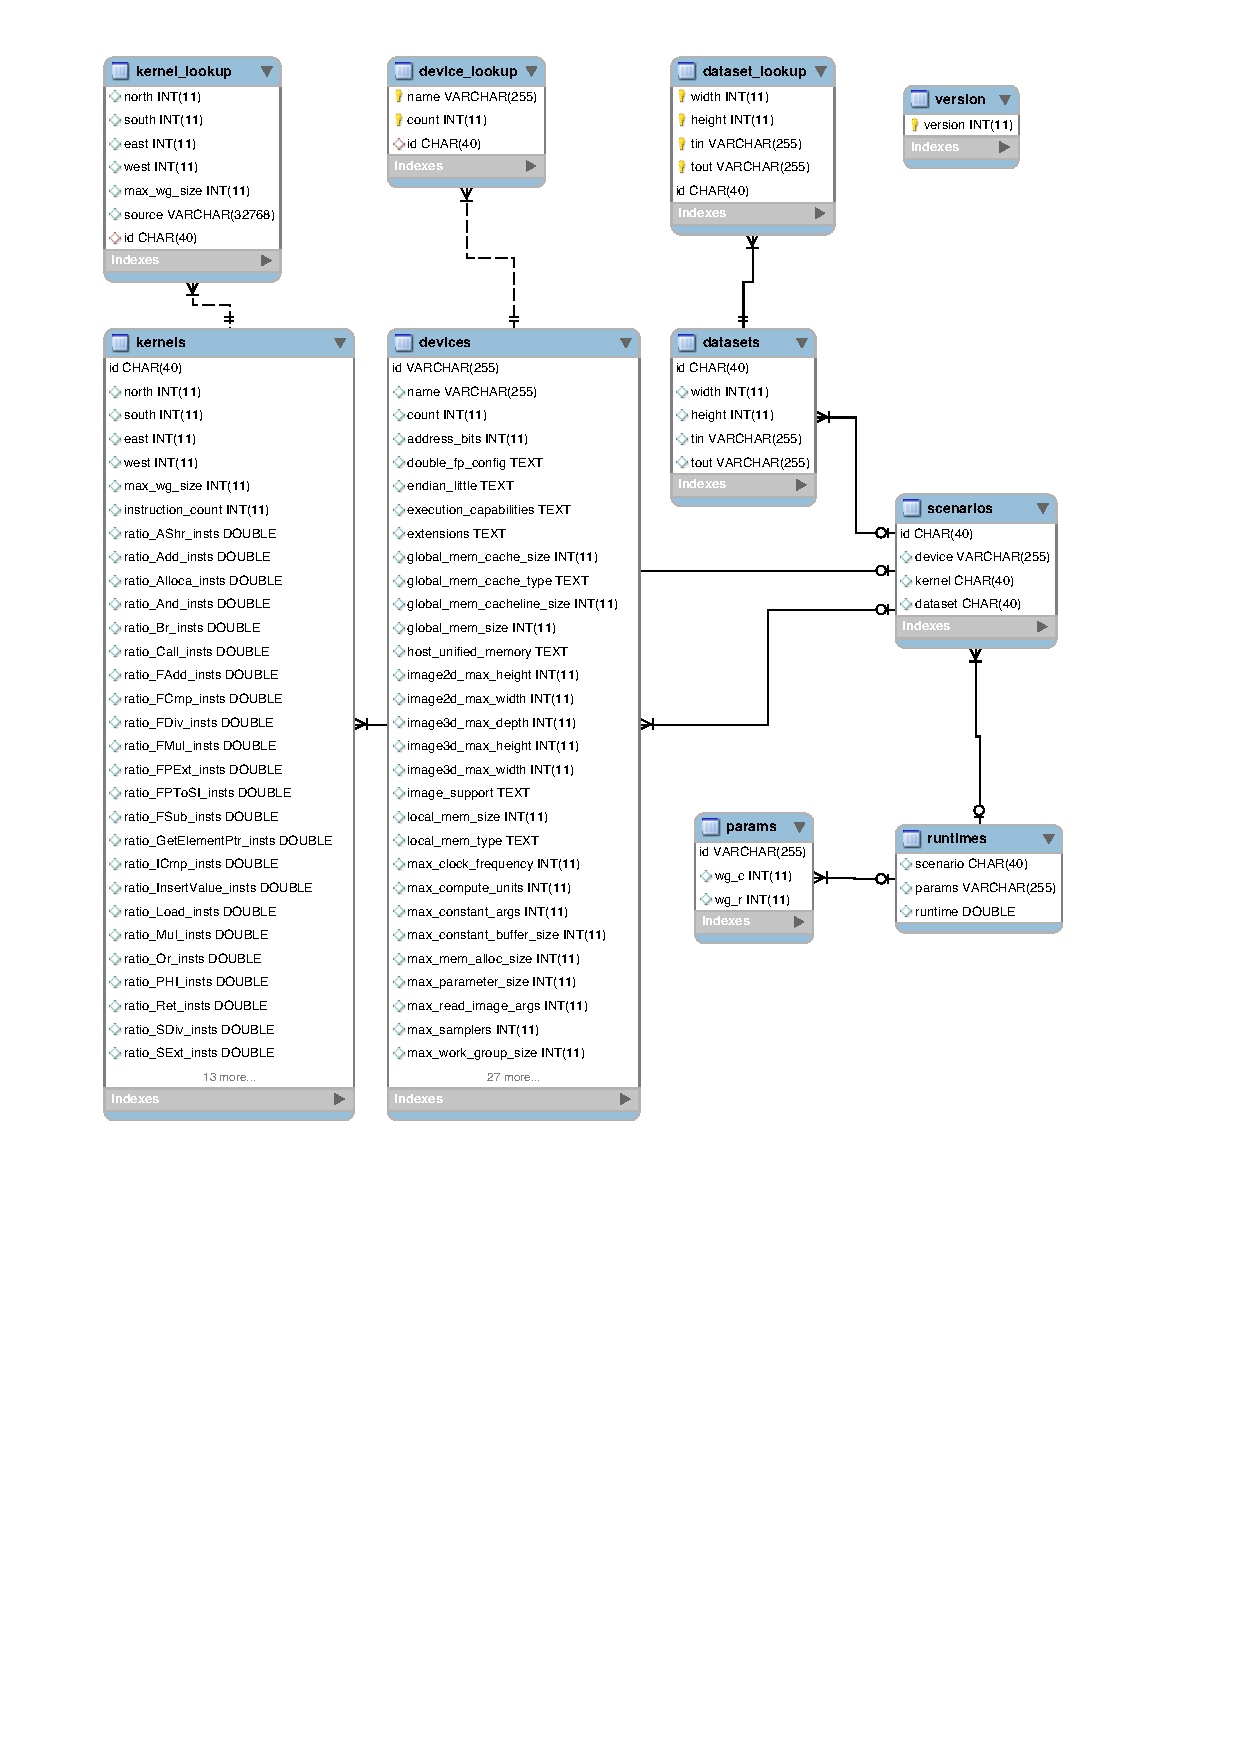
\includegraphics[width=.75\textwidth]{img/omnitune-data-schema.pdf}
\caption{%
  OmniTune SkelCL schema.%
}
\label{fig:omnitune-system-flow}
\end{figure}


\section{Summary}

\TODO{\ldots}
